\section{Navier-Stokes Simulation}
\label{sec:02_Navier-Stokes_Simulation}

The main goal of this section of the project is to extend the \textbf{\lifex} library  with new features, making it a more general-purpose and high-performance simulation framework. Specifically, the work focuses on integrating one-equation \textbf{RANS turbulence model} (Spalart-Allmaras) into the existing incompressible \textbf{Navier-Stokes solver} (NS), enabling the simulation of turbulent flows in external aerodynamic configurations.

\subsection{\textbf{\lifex} Implementation}
\label{sec:lifex_impl}

As detailed by \citet{africa2024lifex}, \textbf{\lifex} is an open-source \cpp library built on top of \dealii, originally designed for life-science applications such as cardiac and cardiovascular fluid dynamics. While the library provides a robust and well-structured finite element infrastructure, its original focus on biomedical applications necessitated several non-trivial adaptations to extend it to external aerodynamic flows.\\

This work addressed four primary challenges:
\begin{itemize}
    \item[-] adapting the solver and utility functions, originally designed for three-dimensional problems, to two-dimensional domains (Section \ref{sec:02_2d_imp});
    \item[-] integrating the one-equation Spalart-Allmaras (SA) RANS model to account for turbulent effects (Section \ref{sec:02_turb_mod});
    \item[-] implementing specialized conditions for aerodynamic simulations, including wall functions and far-field boundaries (Section \ref{sec:02_bc})
    \item[-] developing a residual-based post-processing utility to compute lift and drag forces (Section \ref{sec:02_coef}).
\end{itemize}
\vspace{2ex}
The following sections detail the implementation of each of these components.

% ---------------------------------------------------------------

\subsubsection{2D Implementation}
\label{sec:02_2d_imp}

While the \textbf{\lifex} \texttt{FluidDynamics} solver is templated on the spatial dimension \texttt{dim} through the \dealii convention, its original test cases and utilities were primarily designed for three-dimensional domains. Extending the framework to 2D involved adapting three key components: the finite element function space, the calculation of vorticity and the computation of the wall distance field.

\paragraph{Function space and triangulation}

The SA solver uses \textbf{$Q_1$ finite elements} (\texttt{FE\_Q} of degree 1)
on the same triangulation as the NS solver:
\begin{equation}
  \tilde{\nu}_h \in V_h
  = \bigl\{\,v \in H^1(\Omega) \;\big|\; v\big|_{\partial\Omega_D} = g_D\bigr\}
\end{equation}
On the implementation side, the SA Degree of Freedom (DoF) handler (\texttt{dof\_handler\_sa\_}) is independent from the NS one (\texttt{dof\_handler}), in a way that the two systems have disjoint degrees of freedom without altering the block structure of the Navier-Stokes system. The shared triangulation object is the key architectural choice that allows both DoF handlers to be iterated in lockstep during matrix assembly.

\paragraph{Vorticity in 2D}

The modified vorticity $\tilde{S}$ entering the SA production term requires
the vorticity magnitude $S = |\boldsymbol{\omega}|$. In three dimensions, this is computed as $S = |\nabla \times \mathbf{u}|$.\\

In a 2D context, it simplifies to the absolute value of the scalar curl:
\begin{equation}
  S = \left|\frac{\partial u_y}{\partial x} - \frac{\partial u_x}{\partial y}\right|
\end{equation}
which is extracted from the velocity gradient tensor $\nabla \mathbf{u}^{n+1}$ interpolated at quadrature points via\\ \texttt{fe\_values\_ns\_.get\_function\_gradients}.

\paragraph{Wall distance in 2D}


The wall distance $d(\mathbf{x})$ is computed once during \texttt{setup()} via a parallel algorithm. Each MPI rank collects the barycenters of boundary faces tagged as \texttt{prm\_wall\_tag\_} (airfoil surface), serializes them into a flat \texttt{double} array of size $N_\text{face,loc} \times 2$, and participates in a global \texttt{MPI\_Allgatherv} to build the complete set $\{\mathbf{c}_w\}_{w=1}^{N_\text{face,tot}}$.\\

The distance at every locally owned SA node $i$ is then:
\begin{equation}
  d_i = \max\!\left(\,\min_{w} \|\mathbf{x}_i - \mathbf{c}_w\|_2,\;
  10^{-12}\right)
\end{equation}
where the lower clamp prevents division by zero for nodes sitting exactly on the wall boundary.\\

The result is stored in \texttt{wall\_distance\_ghosted\_}, a Trilinos ghosted vector indexed on \texttt{dof\_handler\_sa\_}, following the standard pattern:
\begin{enumerate}
  \item write into an owned vector and call
        \texttt{compress(VectorOperation::insert)}.
  \item copy owned $\to$ ghosted to propagate ghost entries across MPI ranks.
\end{enumerate}
The overall complexity per rank is $O(N_\text{face,tot} \cdot N_\text{nodes,loc})$, which is acceptable for the 2D meshes used in the airfoil example.

% ---------------------------------------------------------------
\subsubsection{Turbulence Model}
\label{sec:02_turb_mod}

To enable the simulation of turbolent flows, the framework was extended with the one-equation SA RANS model, introduced by \cite{spalart1992}.
This model introduces a transport equation for a scalar variable known as the \emph{modified kinematic viscosity}, $\tilde{\nu}$:
\begin{equation}
\boxed{
  \frac{\partial \tilde{\nu}}{\partial t} + \mathbf{u} \cdot \nabla \tilde{\nu}
  =
  \underbrace{c_{b1}\tilde{S}\tilde{\nu}}_{\text{production}}
  -\underbrace{c_{w1}f_w\!\left(\frac{\tilde{\nu}}{d}\right)^{\!2}}_{\text{destruction}}
  +\underbrace{\frac{1}{\sigma}\Bigl[
     \nabla\cdot\bigl((\nu+\tilde{\nu})\nabla\tilde{\nu}\bigr)
     + c_{b2}|\nabla\tilde{\nu}|^2
   \Bigr]}_{\text{diffusion + cross-diffusion}}
}
\end{equation}

The model constants (Table \ref{tab:sa_constants}) follow the standard set by \textbf{NASA Turbulence Modeling Resource (TMR)} without the $f_{t2}$ trip term.

\begin{table}[h!]
  \centering
  \caption{Spalart-Allmaras model constants based on the NASA TMR standard.}
  \label{tab:sa_constants}
  \begin{tabular}{lll}
    \hline
    Constant & Value & Role \\
    \hline
    $c_{b1}$ & $0.1355$ & production coefficient \\
    $c_{b2}$ & $0.622$  & cross-diffusion coefficient \\
    $\sigma$  & $2/3$    & turbulent Prandtl number \\
    $\kappa$  & $0.41$   & von K\'arm\'an constant \\
    $c_{v1}$ & $7.1$    & viscous damping \\
    $c_{w1}$ & $\approx 3.2391$ & destruction (derived from log-law consistency) \\
    $c_{w2}$ & $0.3$    & regularization in $f_w$ \\
    $c_{w3}$ & $2.0$    & regularization in $f_w$ \\
    \hline
  \end{tabular}
\end{table}

\paragraph{Closure functions}

The model relies on a set of non-linear closure functions to relate $\tilde{\nu}$ to the turbulent eddy viscosity. Defining the viscosity ratio $\chi = \tilde{\nu}/\nu$, these functions are:
\[
  f_{v1}(\chi) = \frac{\chi^3}{\chi^3 + c_{v1}^3}, \qquad
  f_{v2}(\chi) = 1 - \frac{\chi}{1 + \chi f_{v1}(\chi)},
\]
\[
  \tilde{S} = \max\!\left(S + \frac{\tilde{\nu}\,f_{v2}}{\kappa^2 d^2},\;
  10^{-10}\right),
\]
\[
  r = \min\!\left(\frac{\tilde{\nu}}{\tilde{S}\,\kappa^2 d^2},\; 10\right),
  \quad
  g = r + c_{w2}(r^6 - r),
  \quad
  f_w(g) = g\left(\frac{1+c_{w3}^6}{g^6+c_{w3}^6}\right)^{1/6},
\]
The final turbulent eddy viscosity, $\nu_t$, which modifies the momentum equations, is then computed as:
\[
  \nu_t = \tilde{\nu}\,f_{v1}(\chi).
\]

\paragraph{Time discretization and operator splitting.}

To solve the coupled Navier-Stokes and Spalart-Allmaras system, this is advanced at each time step using a \textbf{first-order Lie splitting} scheme (splitting error $O(\Delta t)$). This approach is consistent with the first-order BDF1 time integration used for both solvers.\\

Given the state $(\mathbf{u}^n, p^n, \tilde{\nu}^n)$ at time $t^n$, the solution at $t^{n+1}$ is obtained in two steps:
\begin{enumerate}[itemsep=2ex, topsep=2ex]
  \item the \textbf{NS step} solve the momentum and continuity equations with the with effective viscosity frozen at $\tilde{\nu}^n$:
  \begin{equation*}
    \rho\frac{\mathbf{u}^{n+1}-\mathbf{u}^n}{\Delta t}
    + \rho(\mathbf{u}^* \cdot \nabla)\mathbf{u}^{n+1}
    - \nabla\cdot\!\left(2\mu_\text{eff}^n\,\nabla^S\mathbf{u}^{n+1}\right)
    + \nabla p^{n+1} = \mathbf{0},
  \end{equation*}
  where $\mu_{\text{eff}}^n = \mu + \nu_t(\tilde{\nu}^n)$ is \textit{explicit} with respect to the SA variable;
  \item the \textbf{SA step} solve the transport equation using the velocity field $\mathbf{u}^{n+1}$ just computed and a semi-implicit linearization:
  \[
    \frac{\tilde{\nu}^{n+1}-\tilde{\nu}^n}{\Delta t}
    + \mathbf{u}^{n+1}\cdot\nabla\tilde{\nu}^{n+1}
    = c_{b1}\tilde{S}^n\tilde{\nu}^{n+1}
    - c_{w1}f_w^n\frac{\tilde{\nu}^n}{d^2}\tilde{\nu}^{n+1}
    + \frac{\nu+\tilde{\nu}^n}{\sigma}\Delta\tilde{\nu}^{n+1}
    + \frac{c_{b2}}{\sigma}|\nabla\tilde{\nu}^n|^2.
  \]
\end{enumerate}
\vspace{2ex}
The linearization strategy is the following:
\begin{itemize}[itemsep=2ex, topsep=2ex]
  \item[-] the \textbf{production} is treated implicitly using a Picard iteration. $\tilde{S}^n$ is frozen and $\tilde{\nu}^{n+1}$ appears linearly in the matrix (stabilizing for $\tilde{S}^n > 0$);
  \item[-] the \textbf{destruction}is linearized around $\tilde{\nu}^n$. The coefficient $c_{w1}f_w^n\tilde{\nu}^n/d^2$ enters as a positive reaction term, ensuring coercivity;
  \item[-] about the \textbf{Diffusion}, the coefficient $(\nu+\tilde{\nu}^n)/\sigma$ is explicit while $\Delta\tilde{\nu}^{n+1}$ is implicit;
  \item[-] about the \textbf{Cross-diffusion}, $c_{b2}/\sigma\,|\nabla\tilde{\nu}^n|^2$ is fully explicit and moved to the right-hand side.
\end{itemize}

\paragraph{Weak formulation and SUPG stabilization}

To handle the advection-dominated nature of the SA equation, the weak form is stabilized using the \textbf{Streamline-Upwind Petrov-Galerkin} (SUPG) method.\\

Multiplying by the SUPG test function $\psi_h = v_h + \tau_\text{SUPG}\,\mathbf{u}\cdot\nabla v_h$ and integrating over $\Omega$, the discrete linear system components become:
\[
  A^K_{ij} = \int_K \!\left[
    \psi_i \frac{\phi_j}{\Delta t}
    + \psi_i(\mathbf{u}\cdot\nabla\phi_j)
    + D\,\nabla\phi_i\cdot\nabla\phi_j
    - \psi_i\,c_{b1}\tilde{S}^n\,\phi_j
    + \psi_i\,c_{w1}f_w^n\frac{\tilde{\nu}^n}{d^2}\,\phi_j
  \right]dK,
\]
\[
  b^K_i = \int_K \psi_i\!\left[
    \frac{\tilde{\nu}^n}{\Delta t}
    + \frac{c_{b2}}{\sigma}|\nabla\tilde{\nu}^n|^2
  \right]dK,
\]
where $D = (\nu+\tilde{\nu}^n)/\sigma$.\\

The stabilization parameter$ \tau_\text{SUPG}$ is defined locally for each cell $K$ as:
\[
  \tau_\text{SUPG} = \frac{1}{\displaystyle\sqrt{
    \left(\frac{2}{\Delta t}\right)^{\!2}
    +\left(\frac{2|\mathbf{u}|}{h_K}\right)^{\!2}
    +\left(\frac{4D}{h_K^2}\right)^{\!2}
  }},
\]
where $h_K$ is the minimum vertex distance of cell $K$.\\

% MODIFICA 1 — clamp post-solve
\paragraph{Physical bound enforcement.}

After each linear solve, a physical bound is enforced on the owned vector before updating the ghosted copy (the ordering \texttt{compress(VectorOperation::insert)} $\to$ ghosted copy is mandatory):
\begin{itemize}
  \item[-] negative values ($\tilde{\nu} < 0$) are clamped to $0.0$, since turbulent viscosity cannot be negative (SA physical bound);
  \item[-] \texttt{NaN} values ($\tilde{\nu} = \texttt{NaN}$) are reset to $\tilde{\nu}_\infty$ (freestream value) rather than zero, so that the affected cell remains active and self-corrects over subsequent time steps, avoiding a permanently "dead" region in the domain.
\end{itemize}

% MODIFICA 2 — bisection
\paragraph{Adaptive time-stepping and bisection.}

The bisection mechanism of \texttt{FluidDynamics} is fully supported.\\

\texttt{try\_timestep\_with\_bisection} is declared \texttt{virtual} in the
base class, and \texttt{FluidDynamicsSA} overrides it by calling
\texttt{sa\_solver.take\_snapshot()} before each attempt and
\texttt{sa\_solver.restore\_snapshot()} on failure, ensuring that the SA
state $\tilde{\nu}^n$ is rolled back consistently at every bisection level.

% ---------------------------------------------------------------
\subsubsection{Boundary Conditions}
\label{sec:02_bc}

The implementation handles three distinct boundary condition types (the airfoil wall, the farfield inlet and the outlet boundaries) imposed on the SA variable each with a different physical motivation.

\paragraph{Wall-resolved (low-Re regime).}
A homogeneous Dirichlet condition is applied on the airfoil surface:
$\partial\Omega_\text{wall}$:
\begin{equation}
  \tilde{\nu} = 0 \quad \text{on } \partial\Omega_\text{wall}.
\end{equation}
This is the physically correct condition in the viscous sublayer, as the viscosity $\nu_t$ must vanish as the distance to the wall $d \to 0$.

\paragraph{Wall functions (high-Re regime).}

When the first mesh node is at $y^+ > 5$ (unresolved sublayer), a non-homogeneous Dirichlet condition is derived from the \textbf{log-law}:
\begin{enumerate}[topsep=2ex]
\item the friction velocity is estimated via Schlichting's flat-plate formula:
\[
  C_f = \frac{0.026}{Re^{0.143}} \qquad\text{and}\qquad
  u_\tau = U_\infty\sqrt{C_f/2}
\]
\item the wall-normal distance of the first node is converted to wall units:
\[
  y^+ = \frac{d_\text{node}\, u_\tau}{\nu}.
\]
\item a switch criterion at $y^+_\text{sw} = 11.06$ separates the sublayer from the log-layer:
\[
  \tilde{\nu}_\text{wall} =
  \begin{cases}
    0 & \text{if } y^+ < y^+_\text{sw}, \\
    \text{root of } \nu_t(\tilde{\nu}) = \nu\kappa y^+ & \text{otherwise.}
  \end{cases}
\]
\item the inversion of $\nu_t(\tilde{\nu}) = \tilde{\nu}\,f_{v1}(\tilde{\nu}/\nu)$ is performed with a \textbf{fixed-point iteration}:
\[
  \tilde{\nu}^{(k+1)} = \frac{\nu\kappa y^+}{f_{v1}\!\left(\tilde{\nu}^{(k)}/\nu\right)},
  \quad k = 0,\ldots,4,
\]
which converges in 5 iterations due to the monotonicity of $f_{v1}$.
\end{enumerate}

\paragraph{Inlet and farfield.}
A Dirichlet condition with freestream value is imposed:
\begin{equation}
  \tilde{\nu} = \tilde{\nu}_\infty \in [3\nu,\, 5\nu]
  \quad \text{on } \partial\Omega_\text{inlet} \cup \partial\Omega_\text{farfield}.
\end{equation}

\paragraph{Outlet.}
No condition is explicitly imposed: the natural Neumann condition
$\partial_n\tilde{\nu} = 0$ arises automatically from the boundary term
produced by integration by parts of the diffusion operator in the weak form.

% ---------------------------------------------------------------
\subsubsection{Aerodynamic Coefficients (Residual-Based Approach)}
\label{sec:02_coef}

Lift and drag coefficients are computed at the end of each time step via a
\textbf{residual-based boundary force method}, using the
\texttt{FluidDynamics::compute\_force(tag)} method available in \textbf{\lifex},
which integrates the full stress tensor over the boundary face with the
prescribed tag (airfoil wall):
\begin{equation}
  \mathbf{F} = \int_{\partial\Omega_\text{wall}}
  \boldsymbol{\sigma}\cdot\mathbf{n}\, d\Gamma,
  \qquad
  \boldsymbol{\sigma} = -p\,\mathbf{I} + 2\mu_\text{eff}\,\nabla^S\mathbf{u}.
\end{equation}

\begin{figure}[h!]
    \centering
    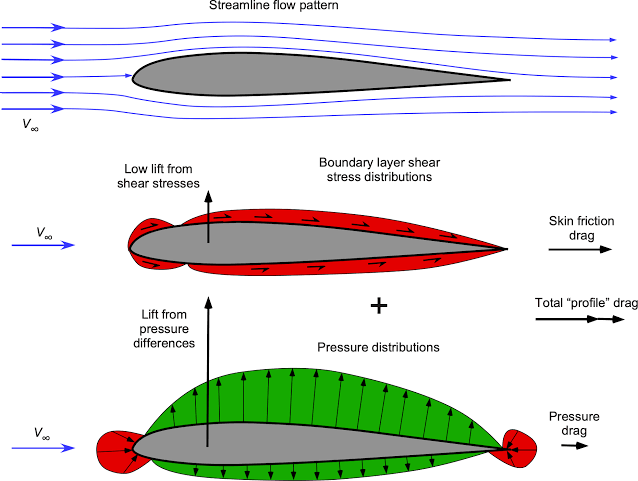
\includegraphics[width=0.5\linewidth]{Images/Chapter02/image.png}
    \caption{Aerodynamic forces on an airfoil. Source: Eagle Pubs}
    \label{fig:aerodynamic_forcex}
\end{figure}

\vspace{2ex}
As illustrated in Figure \ref{fig:aerodynamic_forcex}, the Cartesian force components $(F_x, F_y)$ are projected into the aerodynamic reference frame using the angle of attack $\alpha$:
\begin{equation}
  D = F_x\cos\alpha + F_y\sin\alpha, \qquad
  L = -F_x\sin\alpha + F_y\cos\alpha.
\end{equation}
\vspace{2ex}

The forces are normalized by the dynamic pressure $q_\infty$ and the
reference surface $S_\text{ref}$ (which corresponds to the chord length in 2D simulations):
\begin{equation}
  q_\infty = \tfrac{1}{2}\rho U_\infty^2, \qquad
  C_L = \frac{L}{q_\infty S_\text{ref}}, \qquad
  C_D = \frac{D}{q_\infty S_\text{ref}}.
\end{equation}

\paragraph{Implementation details}

This procedure is encapsuled in a header-only utility class \texttt{AerodynamicCoefficientsEvaluator} that exposes a single method:
\begin{lstlisting}[style=cppstyle, caption={Method from \texttt{AerodynamicCoefficientsEvaluator}.}]
compute_coefficients(tag, density, U_inf, S_ref, alpha)
\end{lstlisting}
It is registered as a callback via \texttt{FluidDynamics::set\_end\_timestep\_callback}, so it executes
automatically after each successful NS time step. Results are then appended to a CSV file (\texttt{force.csv}) with columns \texttt{time, F\_lift, F\_drag, C\_L, C\_D}.

% MODIFICA 3 — parametro di configurazione
\subsubsection{Configuration}

The turbulence model is selected via the parameter \texttt{"Turbulence model": "Spalart-Allmaras"} in the JSON configuration file.\\

For backward compatibility, \texttt{FluidDynamicsSA} also accepts the legacy value \texttt{"None"}, overriding it internally with \texttt{Turbulence::SpalartAllmaras} after \texttt{parse\_parameters}.\\

The \texttt{enum class Turbulence} in \texttt{fluid\_dynamics.hpp} was extended accordingly:
\begin{lstlisting}[style=cppstyle, caption={Extension of the class \texttt{Turbolence}.}]
enum class Turbulence { None, VMS_LES, SpalartAllmaras };
\end{lstlisting}

% ---------------------------------------------------------------
\subsection{Computational framework and execution workflow}

This section details the computational environment and the end-to-end workflow established for the simulation.

\subsubsection{HPC platform and software stack}

All simulations were executed on \textbf{Leonardo} at CINECA (Bologna), targeting the \texttt{dcgp\_usr\_prod} partition (Intel Sapphire Rapids nodes, 112~cores per node) under the EuroHPC allocation \texttt{EUHPC\_D35\_025}, with job submission managed by the SLURM scheduler.\\

The simulation framework is \texttt{LifeX} 2.1, introduced in Section~\ref{sec:lifex_impl}, compiled against \dealii 9.7.1 with \textbf{Trilinos} as the linear-algebra backend, MPICH 4.0 for distributed-memory parallelism, and HDF5 1.14.5 for field output in XDMF format. Meshes are generated externally with Gmsh and read by \textbf{\lifex} in MSH~2.2 format.\\

The full software stack is delivered to the compute nodes through an Apptainer image (\texttt{lifex\_env.sif}) maintained by the \textbf{\lifex} developers, which removes the need for any host-level \texttt{module load} of HPC libraries; the build procedure and the rationale behind this choice are detailed in Section~\ref{sec:container_build}.\\

The resources allocated for each run of the simulation campaign are summarized in Table~\ref{tab:hpc_resources}.

\begin{table}[H]
  \centering
  \begin{tabular}{ll}
    \hline
    \textbf{Component} & \textbf{Specification} \\
    \hline
    Cluster & Leonardo @ CINECA (EuroHPC) \\
    Partition & \texttt{dcgp\_usr\_prod} \\
    CPU & Intel Sapphire Rapids \\
    Cores per node & 112 \\
    MPI ranks per simulation & 8 \\
    Wall-time per run & up to 24~h \\
    Software stack & LifeX 2.1 / deal.II 9.7.1 / Trilinos / MPICH 4.0 / HDF5 1.14.5 \\
    Container runtime & Apptainer 1.4.5 (image \texttt{lifex\_env.sif}) \\
    \hline
  \end{tabular}
  \caption{Computational resources for the simulation campaign on Leonardo.}
  \label{tab:hpc_resources}
\end{table}


\subsubsection{Containerization and build process}
\label{sec:container_build}

The compute nodes of Leonardo do not expose a pre-configured HPC software stack through the \texttt{module} command, which only loads base system libraries. A native build of \textbf{\lifex} on the cluster would therefore require manually compiling \dealii~9.7 together with all its required backends\footnote{\texttt{Trilinos} (used by \texttt{LinearAlgebraTrilinos} and the \texttt{sacado\_dfad} AD operators), PETSc, p4est, VTK, Boost, and HDF5}, an operation that is both fragile and not portable across nodes. The entire toolchain was therefore packaged into an Apptainer image and executed through the container runtime available on the compute nodes (Apptainer~1.4.5), so that the build environment is identical to the execution environment.\\

Identifying an image that simultaneously satisfies all \textbf{\lifex} dependencies required iterating over several candidates, summarized in Table~\ref{tab:container_attempts}, encountering a series of incompatibilities:
\begin{itemize}[itemsep=2ex, topsep=2ex]
    \item[-] the Spack stack pre-installed on Leonardo provides \texttt{dealii@9.6.2}, but only with the \texttt{\textasciitilde{}trilinos} variant, which is incompatible with \textbf{\lifex}~2.1;
    \item[-] the official \texttt{dealii/dealii} Docker images expose \dealii~9.7 with all required backends, but lack the \texttt{boost\_filesystemConfig.cmake} component required by the \textbf{\lifex} CMake configuration;
    \item[-] an earlier MOX \texttt{mk} container shipping \dealii~9.5.1 fails to compile \textbf{\lifex}~2.1 due to API changes in \texttt{get\_mpi\_communicator}, \texttt{CellStatus}, and \texttt{AffineConstraints} that occurred upstream between 9.5 and 9.7
\end{itemize}
The image finally adopted, \texttt{mk-dealiimaster\_latest.sif}, is the MOX MK container with the \dealii module tracking the upstream master branch (\dealii~9.7), together with matching \texttt{vtk}, \texttt{boost}, \texttt{trilinos}, \texttt{petsc}, \texttt{p4est}, and \texttt{hdf5} modules, activated inside the container by sourcing \texttt{/u/sw/etc/profile} and loading the relevant modules.

\begin{table}[h!]
  \centering
  \footnotesize
  \begin{tabular}{p{0.27\textwidth} p{0.33\textwidth} p{0.30\textwidth}}
    \hline
    \textbf{Stack} & \textbf{Components} & \textbf{Outcome} \\
    \hline
    Spack \texttt{dealii@9.6.2} (Leonardo) &
    deal.II \texttt{\textasciitilde{}trilinos}, PETSc, MPICH &
    Missing Trilinos/Sacado required by LifeX 2.1 \\
    \texttt{dealii/dealii} Docker images (\texttt{v9.7.1-jammy}, \texttt{master-jammy}, \texttt{v9.7.1-noble}) &
    deal.II 9.7.1 with Trilinos, PETSc, p4est, VTK, HDF5 &
    \texttt{boost\_filesystemConfig.cmake} missing in the image \\
    MOX \texttt{mk} container (deal.II 9.5.1) &
    deal.II 9.5.1, Boost 1.76, VTK, HDF5 &
    API mismatch: LifeX 2.1 requires deal.II $\geq$ 9.7 \\
    \texttt{mk-dealiimaster\_latest.sif} &
    MK toolchain with deal.II master ($\geq$ 9.7), Boost, VTK, Trilinos, PETSc, p4est, HDF5 &
    \textbf{Adopted} for the simulation campaign \\
    \hline
  \end{tabular}
  \caption{Container strategies evaluated for building LifeX on Leonardo.}
  \label{tab:container_attempts}
\end{table}

\vspace{2ex}

The CMake configuration is invoked through \texttt{apptainer exec --cleanenv --bind}, which strips host environment contamination and mounts the workspace inside the container. Because the simulation campaign is purely two-dimensional, the build is configured with \texttt{-DLIFEX\_DIM=2} and restricted to the two example targets actually used, \texttt{example\_fluid\_dynamics\_airfoil} and \texttt{example\_fluid\_dynamics\_external\_flow}. A global \texttt{make all} cannot be used in 2D because some files in the test suite (e.g.\ \texttt{tests/multidomain\_laplace/laplace.cpp}) rely on overloads of \texttt{GridTools::rotate} that exist only for three-dimensional triangulations, and the resulting compilation error stops the whole build.\\
The complete build script is reported in Listing~\ref{lst:job_build}.

\begin{lstlisting}[style=bashstyle, caption={SLURM build script for LifeX on Leonardo (\texttt{job\_build\_leonardo.sh}). The Apptainer image is invoked through the legacy \texttt{singularity} command alias.}, label={lst:job_build}]
#!/bin/bash
#SBATCH -A EUHPC_D35_025
#SBATCH -p dcgp_usr_prod
#SBATCH --time=00:24:00
#SBATCH -N 1
#SBATCH --ntasks-per-node=112
#SBATCH --job-name=lifex_build

set -euo pipefail

WORK_DIR="$HOME/Ice_acceleration_model_on_airplane_wing"
SIF="${WORK_DIR}/containers/mk-dealiimaster_latest.sif"
SRC_SUBDIR="external/lifex-public"
BUILD_SUBDIR="external/lifex-public/build_2d"

rm -rf "${WORK_DIR}/${BUILD_SUBDIR}"

singularity exec --cleanenv \
  --bind "${WORK_DIR}:/work" \
  --bind /dev/shm:/dev/shm \
  "${SIF}" bash -c "
    source /u/sw/etc/profile
    module load gcc-glibc dealii vtk

    cmake -B /work/${BUILD_SUBDIR} -S /work/${SRC_SUBDIR} \
      -DCMAKE_BUILD_TYPE=Release \
      -DLIFEX_DIM=2 \
      -DDEAL_II_DIR=\${mkDealiiPrefix} \
      -DLin_ALG=Trilinos

    cmake --build /work/${BUILD_SUBDIR} \
      --target example_fluid_dynamics_airfoil \
                example_fluid_dynamics_external_flow \
      -j 112
  "
\end{lstlisting}

\subsubsection{Mesh generation and pre-processing pipeline}\label{sec:mesh}

The computational meshes are generated with Gmsh from parametric \texttt{.geo} scripts, driven by a set of Python generators (\texttt{generate\_geo*.py}, \texttt{naca\_generator\_v*.py}) that expose the airfoil profile (NACA~0006 through NACA~0018), the domain extent, and the boundary-layer structure as input parameters.\\

The resulting mesh is hybrid: a structured layer of quadrilaterals wraps the airfoil surface to resolve the boundary layer, while the outer region is filled with unstructured triangles. Boundary entities follow a fixed tagging convention (\texttt{1}~=~inlet, \texttt{2}~=~outlet, \texttt{3}~=~airfoil wall) matching the tags expected by the \textbf{\lifex} configuration (Section~\ref{sec:lifex_impl}), and the mesh is exported in the MSH~2.2 format read natively by \dealii.\\

In accordance with the wall-resolved turbulence modeling approach described in Section~\ref{sec:02_bc}, the near-wall region is carefully refined. The height of the first cell layer is adjusted until the estimated dimensionless wall distance satisfies the criterion $y^+ \lesssim 1$ at a Reynolds number of $\mathrm{Re}=10^6$. This ensures that the use of a homogeneous Dirichlet condition for $\tilde{\nu}$ is physically valid.\\

Because a single malformed mesh wastes hours of allocated CPU time, every mesh is screened by a pre-processing pipeline before submission. Four independent Python checks are run in sequence:
\begin{itemize}[itemsep=2ex, topsep=2ex]
  \item[-] \texttt{mesh\_info.py} reports the node and element counts grouped by element type and physical tag and verifies that the inlet, outlet, and airfoil tags are all present;
  \item[-] \texttt{check\_extents.py} computes the bounding box of each tagged boundary, confirming that the inlet, outlet and airfoil entities are positioned where the geometry expects them;
  \item[-] \texttt{check\_jacobians.py} reads the mesh through \texttt{meshio} and computes the signed area of every quadrilateral via the cross product of its diagonals, flagging inverted or non-convex cells that would produce a negative Jacobian;
  \item[-] \texttt{check\_yplus.py} estimates the wall-normal $y^+$ at the first node by measuring the height of the cells adjacent to the airfoil edges and applying a flat-plate skin-friction correlation ($u_\tau/U_\infty \approx 0.036$), consistent with the estimate in Section~\ref{sec:02_bc}.
\end{itemize}
Any mesh that fails one or more of these checks is automatically discarded and regenerated. An example of a mesh that has passed this quality control pipeline, used for the NACA~0012 simulations, is shown in Figure~\ref{fig:mesh}.

\begin{figure}[!htbp]
  \centering
  \subfloat[Overall domain]{
\includegraphics[width=0.45\textwidth]{Chapter02/mesh_overview.png}}
  \hfill
  \subfloat[Leading edge detail]{
\includegraphics[width=0.45\textwidth]{Chapter02/mesh_LE_zoom.png}}
  \caption{Computational mesh for the NACA~0012 airfoil. (a) Overall domain, with a structured quadrilateral boundary layer around the profile and an unstructured triangular outer region. (b) Detail of the wall-resolved boundary layer at the leading edge, refined to give $y^+ \lesssim 1$ at $\mathrm{Re}=10^6$.}
  \label{fig:mesh}
\end{figure}

\subsubsection{Simulation execution and post-processing}
\label{sec:execution}

Each simulation is launched as a single-node SLURM job that runs the \textbf{\lifex} executable inside the Apptainer container with \texttt{mpirun -n 8}, distributing the mesh across eight MPI ranks on the \texttt{dcgp\_usr\_prod} partition.\\

The workspace is bind-mounted into the container and the run-time configuration is supplied as a JSON file, following the parameter structure described in Section~\ref{sec:lifex_impl}: the turbulence model is activated through \texttt{"Turbulence model": "Spalart-Allmaras"}, and the Reynolds number is set implicitly through the kinematic viscosity ($\nu = 10^{-6}$ with $U_\infty = 1$ and chord $c = 1$, giving $\mathrm{Re} = 10^6$). Before execution, the configuration file is copied into the run directory \texttt{output/run\_\$\{SLURM\_JOB\_ID\}/} as \texttt{config\_used.json}, so that every result remains paired with the exact parameters that produced it.\\

During the run, the solver generates two primary forms of output: a time history of the aerodynamic coefficients, which is appended to \texttt{force.csv}, and the full velocity, pressure, and turbulent-viscosity fields, saved as HDF5 files with corresponding XDMF descriptors for visualization in ParaView. The complete SLURM submission script orchestrating this process is reported in Listing~\ref{lst:job_run}.\\

\begin{lstlisting}[style=bashstyle,
  caption={SLURM run script for a single simulation (\texttt{job\_run\_leonardo.sh}).},
  label={lst:job_run}]
#!/bin/bash
#SBATCH -A EUHPC_D35_025
#SBATCH -p dcgp_usr_prod
#SBATCH --time=24:00:00
#SBATCH -N 1
#SBATCH --ntasks-per-node=8
#SBATCH --job-name=lifex_run
#SBATCH -o output/run_%j/solver.log

set -euo pipefail

WORK_DIR="$HOME/Ice_acceleration_model_on_airplane_wing"
SIF="${WORK_DIR}/containers/mk-dealiimaster_latest.sif"
EXEC="/work/external/lifex-public/build_2d/examples/fluid_dynamics_airfoil
      /lifex_example_fluid_dynamics_airfoil"
CONFIG="/work/cases/naca0012/config_new_method.json"
RUN_DIR="${WORK_DIR}/output/run_${SLURM_JOB_ID}"

mkdir -p "${RUN_DIR}"
cp "${WORK_DIR}/cases/naca0012/config_new_method.json" "${RUN_DIR}/config_used.json"

singularity exec --cleanenv \
  --bind "${WORK_DIR}:/work" \
  --bind /dev/shm:/dev/shm \
  "${SIF}" bash -c "
    source /u/sw/etc/profile
    module load gcc-glibc dealii vtk
    export LD_LIBRARY_PATH=/work/external/lifex-public/build_2d/lib:\$LD_LIBRARY_PATH

    cd /work/output/run_${SLURM_JOB_ID}
    mpirun -n 8 ${EXEC} ${CONFIG}
  "
\end{lstlisting}

The field output is inspected in ParaView, while the coefficient time histories are plotted with the \texttt{plot\_forces.py} script (matplotlib with the \texttt{Agg} backend, so that figures are rendered without a display on the compute nodes).\\

Figures~\ref{fig:cp} and \ref{fig:vorticity} show representative output for the NACA~0012 at $\alpha = 4^\circ$ and $\mathrm{Re} = 10^6$. The pressure coefficient field (Figure~\ref{fig:cp}) exhibits the suction peak on the upper surface near the leading edge that generates the net lift; the velocity field (Figure~\ref{fig:velocity}) shows the flow accelerating over the suction side and the thin viscous wake downstream of the trailing edge; the spanwise vorticity (Figure~\ref{fig:vorticity}) isolates the shed boundary layers in the wake.

\begin{figure}[!htbp]
  \centering
  
\includegraphics[width=0.65\textwidth]{Chapter02/Cp_field.png}
  \caption{Pressure coefficient field around the NACA~0012 at $\alpha = 4^\circ$, $\mathrm{Re} = 10^6$. The suction peak on the upper surface near the leading edge and the stagnation region on the lower side generate the net lift.}
  \label{fig:cp}
\end{figure}

\begin{figure}[!htbp]
  \centering
  \subfloat[Velocity magnitude with superimposed streamlines.]
    {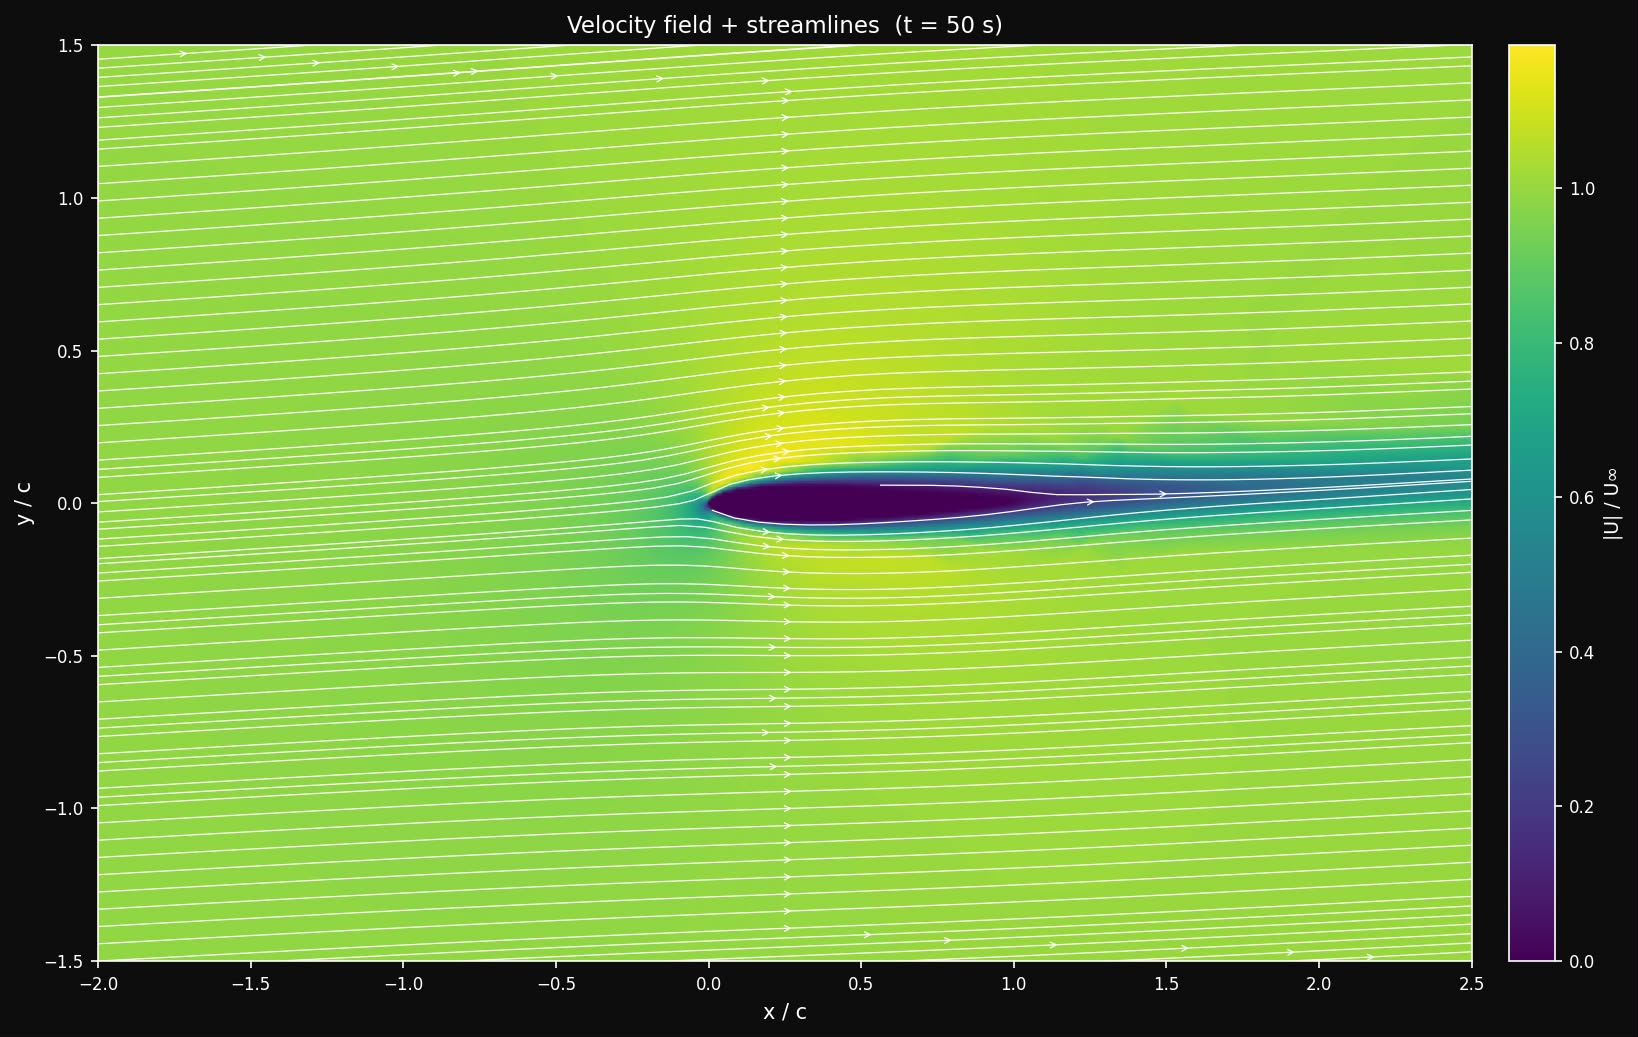
\includegraphics[width=0.45\textwidth]{Images/Chapter02/velocity_streamlines.jpeg}\label{fig:velocity}}
  \hfill
  \subfloat[Spanwise vorticity in the wake.]
    {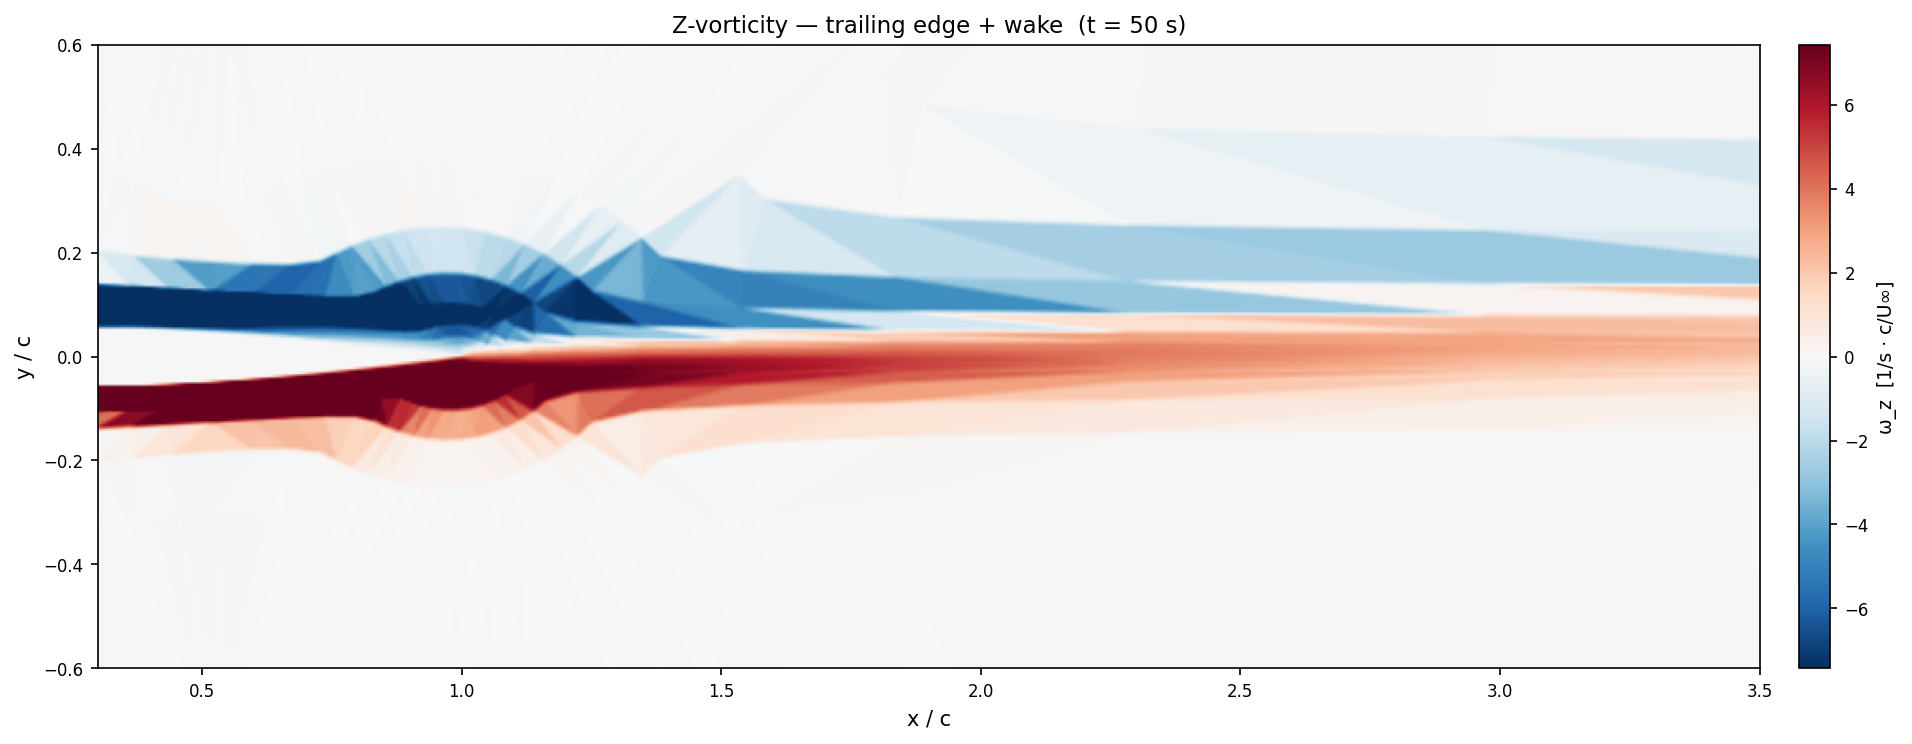
\includegraphics[width=0.45\textwidth]{Images/Chapter02/vorticity_wake.png}\label{fig:vorticity}}
  \caption{Flow field around the NACA~0012 at $\alpha = 4^\circ$, $\mathrm{Re} = 10^6$. (a) The flow accelerates over the suction side and produces a thin viscous wake downstream of the trailing edge. (b) The spanwise vorticity isolates the shed boundary layers.}
\end{figure}

\subsubsection{Dataset generation for the surrogate model}
\label{sec:dataset}

The simulation is not an end in itself: its role is to build the training set for the convolutional surrogate model presented in Section~\ref{sec:03_Convolutional_Neural_Network}.\\

To build a comprehensive dataset, the parameter space was systematically explored. For each airfoil profile in a family of symmetric NACA sections (NACA~0006 to NACA~0018), the angle of attack was swept over the range $\alpha \in \{-14^\circ, -12^\circ, \ldots, +14^\circ\}$ using templated configuration files (\texttt{config\_isa\_aoa\_*.json}).\\

For each configuration, the pipeline produces a single label: the converged lift coefficient, $C_L$. These labels populate the \texttt{Y\_cl} array of the final dataset, which is stored in the compressed NumPy format (\texttt{.npz}). The corresponding inputs are the Signed Distance Function representation of each geometry and the scalar pair of physical parameters $(\mathrm{Re}, \alpha)$.\\

Computing the lift labels with the turbulence-resolved solver, rather than with a low-fidelity panel method, is what allows the surrogate to be trained against high-fidelity data in the high-incidence regime where thin-airfoil theory no longer holds.\\ 

The same workflow extends to the iced-airfoil geometries. A modified leading edge produced by an icing model could be created in future workflows and processed through the identical execution and post-processing chain, so that the dataset can later be augmented with iced profiles without any change to the simulation pipeline. The complete workflow is summarized in Figure~\ref{fig:pipeline}.

\begin{figure}[H]
  \centering
  \begin{tikzpicture}[
    node distance=12mm and 8mm,
    every node/.style={font=\footnotesize},
    stage/.style={
      rectangle, rounded corners=2pt, draw=flowblue, line width=0.6pt,
      fill=flowblue!6, text width=3.5cm, align=center, inner sep=4pt,
      minimum height=13mm},
    data/.style={
      rectangle, rounded corners=2pt, draw=flowslate, line width=0.6pt,
      fill=flowslate!8, text width=3.5cm, align=center, inner sep=4pt,
      minimum height=13mm},
    arr/.style={-{Stealth[length=2.2mm]}, line width=0.7pt, draw=gray!70}
  ]

    \node[data]               (b1) {Configuration: NACA profile, $\alpha$, $\mathrm{Re}$};
    \node[stage, right=of b1] (b2) {Mesh generation\\(Gmsh)};
    \node[stage, right=of b2] (b3) {Quality checks:\\$y^+$, Jacobians, extents};
    \node[stage, below=of b3] (b4) {LifeX on Leonardo:\\SLURM + Apptainer, 8 MPI};
    \node[data,  left=of b4]  (b5) {HDF5/XDMF fields\\$+$ \texttt{force.csv}};
    \node[data,  left=of b5]  (b6) {$C_L$ labels $\rightarrow$\\CNN dataset (Sec.~\ref{sec:03_Convolutional_Neural_Network})};

    \draw[arr] (b1) -- (b2);
    \draw[arr] (b2) -- (b3);
    \draw[arr] (b3) -- (b4);
    \draw[arr] (b4) -- (b5);
    \draw[arr] (b5) -- (b6);

  \end{tikzpicture}
  \caption{End-to-end simulation pipeline (top row left to right, then bottom row right to left). Mesh generation and quality control run interactively on the login node; the solver runs as a SLURM batch job inside the Apptainer container on the compute nodes; the resulting lift coefficients feed the convolutional surrogate model of Section~\ref{sec:03_Convolutional_Neural_Network}.}
  \label{fig:pipeline}
\end{figure}
\FloatBarrier